\documentclass[10pt]{beamer}
\usetheme[
%%% options passed to the outer theme
%    hidetitle,           % hide the (short) title in the sidebar
%    hideauthor,          % hide the (short) author in the sidebar
%    hideinstitute,       % hide the (short) institute in the bottom of the sidebar
%    shownavsym,          % show the navigation symbols
%    width=2cm,           % width of the sidebar (default is 2 cm)
%    hideothersubsections,% hide all subsections but the subsections in the current section
%    hideallsubsections,  % hide all subsections
%    left                % right of left position of sidebar (default is right)
  ]{Aalborg}
  
% If you want to change the colors of the various elements in the theme, edit and uncomment the following lines
% Change the bar and sidebar colors:
%\setbeamercolor{Aalborg}{fg=red!20,bg=red}
%\setbeamercolor{sidebar}{bg=red!20}
% Change the color of the structural elements:
%\setbeamercolor{structure}{fg=red}
% Change the frame title text color:
%\setbeamercolor{frametitle}{fg=blue}
% Change the normal text color background:
%\setbeamercolor{normal text}{bg=gray!10}
% ... and you can of course change a lot more - see the beamer user manual.

\usepackage[utf8]{inputenc}
\usepackage[english]{babel}
\usepackage[T1]{fontenc}
% Or whatever. Note that the encoding and the font should match. If T1
% does not look nice, try deleting the line with the fontenc.

\usepackage[table,xcdraw]{xcolor}
\usepackage{helvet}
\usepackage[spanish]{babel}
\usepackage{tikz}
\usetikzlibrary{shapes,arrows,positioning}

\usepackage{minted}


\usepackage{listings}
\usepackage{color}
\definecolor{codegreen}{rgb}{0,0.6,0}
\definecolor{codegray}{rgb}{0.5,0.5,0.5}
\definecolor{codepurple}{rgb}{0.58,0,0.82}
\definecolor{backcolour}{rgb}{0.95,0.95,0.92}
 
\lstdefinestyle{mystyle}{
    backgroundcolor=\color{backcolour},   
    commentstyle=\color{codegreen},
    keywordstyle=\color{magenta},
    numberstyle=\tiny\color{codegray},
    stringstyle=\color{codepurple},
    basicstyle=\footnotesize,
    breakatwhitespace=false,         
    breaklines=true,                 
    captionpos=b,                    
    keepspaces=true,                 
    numbers=left,                    
    numbersep=5pt,                  
    showspaces=false,                
    showstringspaces=false,
    showtabs=false,                  
    tabsize=2
}
 
\lstset{style=mystyle}


% colored hyperlinks
\newcommand{\chref}[2]{%
  \href{#1}{{\usebeamercolor[bg]{Aalborg}#2}}%
}

\title[Solución a problemas EGEL]% optional, use only with long paper titles
{Solución a problemas EGEL}

\subtitle{v.\ 1.0}  % could also be a conference name

\date{3 de agosto de 2018}

\author[Víctor Medrano Zarazúa] % optional, use only with lots of authors
{
  Víctor Medrano Zarazúa\\
  \href{mailto:vdejesusmedrano@gmail.com}{{\tt vdejesusmedrano@gmail.com}}
}
% - Give the names in the same order as they appear in the paper.
% - Use the \inst{?} command only if the authors have different
%   affiliation. See the beamer manual for an example

\institute[
%  {\includegraphics[scale=0.2]{aau_segl}}\\ %insert a company, department or university logo
  %Dept.\ of Electronic Systems\\
  Universidad del Valle de México\\
  Campus Monterrey
] % optional - is placed in the bottom of the sidebar on every slide
{% is placed on the bottom of the title page
  %Department of Electronic Systems\\
  Universidad del Valle de México\\
  Campus Monterrey
  
  %there must be an empty line above this line - otherwise some unwanted space is added between the university and the country (I do not know why;( )
}

% specify the logo in the top right/left of the slide
\pgfdeclareimage[height=1cm]{mainlogo}{AAUgraphics/UVM} % placed in the upper left/right corner
\logo{\pgfuseimage{mainlogo}}

% specify a logo on the titlepage (you can specify additional logos an include them in 
% institute command below
\pgfdeclareimage[height=1.5cm]{titlepagelogo}{AAUgraphics/UVM} % placed on the title page
%\pgfdeclareimage[height=1.5cm]{titlepagelogo2}{AAUgraphics/aau_logo_new} % placed on the title page
\titlegraphic{% is placed on the bottom of the title page
  \pgfuseimage{titlepagelogo}
%  \hspace{1cm}\pgfuseimage{titlepagelogo2}
}

%\definecolor{UniBlue}{RGB}{255,255,255}

\tikzset{
block/.style={
  draw, 
  fill=blue!20, 
  rectangle, 
  minimum height=3em, 
  minimum width=6em
  },
 gain/.style={
    draw,
    fill=blue!20, 
    isosceles triangle,
    minimum height = 3em,
    isosceles triangle apex angle=60
    },
sum/.style={
  draw, 
  fill=blue!20, 
  circle, 
  },
input/.style={coordinate},
output/.style={coordinate},
pinstyle/.style={
  pin edge={to-,thin,black}
  }
}  

\begin{document}
% the titlepage


%\setbeamercolor{title}{fg=UniBlue}
%\setbeamercolor{normal text}{fg=UniBlue}
%\setbeamercolor{Aalborg}{fg=black,bg=black}


{\aauwavesbg
\begin{frame}[plain,noframenumbering] % the plain option removes the sidebar and header from the title page
  \titlepage
\end{frame}}
%%%%%%%%%%%%%%%%

% TOC
\begin{frame}{Problemas}{}
\tableofcontents
\end{frame}
%%%%%%%%%%%%%%%%
\section{Introducción}
\begin{frame}{Introducción}{}
\begin{block}{Solución a problemas EGEL}
En la siguiente presentación se muestra la solución a problemas EGEL. Además de mostrar la solución al problema, se presentan los conocimientos teóricos necesarios para resolverlo y en algunos casos la comprobación de la solución por medio de software.\\

Si solo le interesa la solución del problema, puede dar clic en la sección de solución de la diapositiva anterior.

\end{block}
\end{frame}

\section{Pregunta 34}
\subsection{Problema}
% motivation for creating this theme
\begin{frame}{Pregunta 34}{Problema}
\begin{block}{Seleccione la ganancia en lazo cerrado que reduce el error en estado estacionario del sistema para una entrada escalón unitario y una función de transferencia en lazo abierto:}
\end{block}
\begin{equation}
    \frac{Y(s)}{U(s)} = \frac{2K}{s^{2}+3s+2}
\end{equation}

\end{frame}

\subsection{Teoría}
% motivation for creating this theme
\begin{frame}{Pregunta 34}{Teoría}
\begin{block}{Diagrama de sistema en lazo abierto}
  %\begin{itemize}
   % \item<1-> In August 2010, I gave a presentation at the European Signal Processing Conference (EUSIPCO) here in Aalborg. For that purpose, I created the AAU sidebar beamer theme.
    
  %\end{itemize}
  \begin{minipage}[t]{\linewidth}
    \hspace*{0\linewidth}
    \vspace*{-0.1\linewidth}
    \rule[0cm]{0pt}{2cm}

  \begin{tikzpicture}[auto,>=latex']
    \node [input, name=input] {};
    %\node [sum, right = of input] (sum) {};
    \node [gain, right = of input] (controller) {K};
    \node [block, right = of controller,
            node distance=1cm] (system) {G(s)};
    % We draw an edge between the controller and system block to 
    % calculate the coordinate u. We need it to place the measurement block. 
    \draw [->] (controller) -- node[name=u] {} (system);
    \node [block, right of=system,  node distance=3cm] (measurements) {H(s)};
    \node [output, right =of measurements] (output) {};
    
    %\node [block, below of=u, node distance=1.8cm] (measurements) {H(s)};

    % Once the nodes are placed, connecting them is easy. 
    \draw [draw,->] (input) -- node {$U(s)$} (controller);
    %\draw [->] (sum) -- node {$E(s)$} (controller);
    
    \draw [->] (system) -- (measurements);
    \draw [->] (measurements) -- node [name=y] {$Y(s)$}(output);
    %\draw [->] (measurements) -| node[pos=0.99] {$-$} 
    %    node [near end] {$y_m$} (sum);
  \end{tikzpicture}
  \end{minipage}

\end{block}
\end{frame}
%%%%%%%%%%%%%%%%

\begin{frame}{Pregunta 34}{Teoría}
\begin{block}{Diagrama de sistema en lazo cerrado}
  %\begin{itemize}
   % \item<1-> In August 2010, I gave a presentation at the European Signal Processing Conference (EUSIPCO) here in Aalborg. For that purpose, I created the AAU sidebar beamer theme.
    
  %\end{itemize}
  \begin{minipage}[t]{\linewidth}
    \hspace*{0.1\linewidth}
    %\vspace*{-0.9\linewidth}
    \rule[2cm]{0pt}{2cm}
  \begin{tikzpicture}[auto,>=latex']
    \node [input, name=input] {};
    \node [sum, right = of input] (sum) {};
    \node [gain, right = of sum] (controller) {K};
    \node [block, right = of controller,
            node distance=1cm] (system) {G(s)};
    % We draw an edge between the controller and system block to 
    % calculate the coordinate u. We need it to place the measurement block. 
    \draw [->] (controller) -- node[name=u] {} (system);
    \node [output, right =of system] (output) {};
    \node [block, below of=u, node distance=1.8cm] (measurements) {H(s)};

    % Once the nodes are placed, connecting them is easy. 
    \draw [draw,->] (input) -- node {$U(s)$} (sum);
    \draw [->] (sum) -- node {$E(s)$} (controller);
    \draw [->] (system) -- node [name=y] {$Y(s)$}(output);
    \draw [->] (y) |- (measurements);
    \draw [->] (measurements) -| node[pos=0.99] {$-$} 
        node [near end] {} (sum);
  \end{tikzpicture}
  \end{minipage}

\end{block}
\end{frame}

%%%%%%%%%%%%%%%%

\begin{frame}{Pregunta 34}{Teoría}
\begin{block}{Análisis del sistema en lazo cerrado}
  \begin{itemize}
    \item<1-> Usando álgebra de bloques se obtienen las ecuaciones para calcular el error $E(s)$ por medio de la entrada $U(s)$ y el comportamiento del sistema ($G(s)$, $H(s)$)
    
    \begin{equation}\label{error}
        E(s) = U(s) - Y(s)H(s)
    \end{equation}
    
    \begin{equation}\label{output}
        Y(s) = K E(s) G(s)
    \end{equation}
    
    \vspace{}
    
    \item<2-> De las ecuaciones \ref{error} y \ref{output} se obtiene que:
    
    \begin{equation}\label{error2}
        E(s) = U(s) - KE(s)G(s)H(s)
    \end{equation}
    
  \end{itemize}
 

\end{block}
\end{frame}

%%%%%%%%%%%%%%%%%%%%%%%%%

\begin{frame}{Pregunta 34}{Teoría}
\begin{block}{Análisis del sistema en lazo cerrado}
  \begin{itemize}
    \item<1-> Factorizamos la ecuación \ref{error2} usando $E(s)$ como factor común y obtenemos:
    
    \begin{equation}\label{error3}
        E(s)[1+KG(s)H(s)] = U(s)
    \end{equation}
    
    \vspace{}
    
    \item<2-> Despejamos $E(s)$ en la ecuación \ref{error3}:
    
    \begin{equation}\label{error4}
        E(s) = \frac{U(s)}{1+KG(s)H(s)}
    \end{equation}
    
  \end{itemize}
 

\end{block}
\end{frame}

%%%%%%%%%%%%%%%%%%%%%%%%%

\begin{frame}{Pregunta 34}{Teoría}
\begin{block}{Error en estado estacionario}
  \begin{itemize}
    \item<1-> La expresión de la ecuación \ref{error4} proporciona la transformada de Laplace de la señal de error para todo el tiempo, permitiendo conocer la evolución de la misma durante toda la respuesta del sistema. Si nos interesa conocer el valor del error en estado estacionario, aplicamos el teorema del valor final:
    
    \begin{equation}\label{teoremavf}
        %e_{\infty} = lim_{t\rightarrow\infty} e(t)
        e_{\infty} = \lim\limits_{t \to \infty} e(t) = \lim\limits_{s \to 0} sE(s)
    \end{equation}
    
    \vspace{}
    
    \item<2-> De la ecuación \ref{error4} y \ref{teoremavf} se obtiene:
    
    \begin{equation}\label{sserror}
        \boxed{e_{\infty} = \lim\limits_{s \to 0} s \frac{U(s)}{1+KG(s)H(s)}}
    \end{equation}
    
  \end{itemize}
 

\end{block}
\end{frame}



%%%%%%%%%%%%%%%%
\subsection{Solución}
% how to modify the theme
{\setbeamercolor{Aalborg}{fg=gray!50,bg=gray}
 \setbeamercolor{sidebar}{bg=red!20}
 \setbeamercolor{structure}{fg=red}
 \setbeamercolor{frametitle}{use=structure,fg=structure.fg}
 \setbeamercolor{normal text}{bg=gray!20}
\begin{frame}{Pregunta 34}{Solución}
  
\begin{block}{Función de transferencia en lazo abierto}
  %\begin{itemize}
   % \item<1-> In August 2010, I gave a presentation at the European Signal Processing Conference (EUSIPCO) here in Aalborg. For that purpose, I created the AAU sidebar beamer theme.
    
  %\end{itemize}
  \begin{minipage}[t]{\linewidth}
    \hspace*{0\linewidth}
    \vspace*{-0.1\linewidth}
    \rule[0cm]{0pt}{2cm}

  \begin{tikzpicture}[auto,>=latex']
    \node [input, name=input] {};
    %\node [sum, right = of input] (sum) {};
    \node [gain, right = of input] (controller) {K};
    \node [block, right = of controller,
            node distance=1cm] (system) {G(s)};
    % We draw an edge between the controller and system block to 
    % calculate the coordinate u. We need it to place the measurement block. 
    \draw [->] (controller) -- node[name=u] {} (system);
    \node [block, right of=system,  node distance=3cm] (measurements) {H(s)};
    \node [output, right =of measurements] (output) {};
    
    %\node [block, below of=u, node distance=1.8cm] (measurements) {H(s)};

    % Once the nodes are placed, connecting them is easy. 
    \draw [draw,->] (input) -- node {$U(s)$} (controller);
    %\draw [->] (sum) -- node {$E(s)$} (controller);
    
    \draw [->] (system) -- (measurements);
    \draw [->] (measurements) -- node [name=y] {$Y(s)$}(output);
    %\draw [->] (measurements) -| node[pos=0.99] {$-$} 
    %    node [near end] {$y_m$} (sum);
  \end{tikzpicture}
  \end{minipage}
  
  \medskip
  
  \begin{itemize}
    \item<1-> Apoyados en el diagrama del sistema en lazo abierto y álgebra de bloques para el problema de la pregunta 34 se obtiene que:
    
    \begin{equation}\label{openloop}
        KG(s)H(s) = \frac{2K}{s^2 + 3s + 2}
    \end{equation}
  \end{itemize}

\end{block}
\end{frame}

%%%%%%%%%%%%%%%%%

\begin{frame}{Pregunta 34}{Solución}
  
\begin{block}{Calcular error en estado estacionario}
  
  \begin{itemize}
    \item<1-> La ecuación \ref{sserror} es la que nos guiará a la solución de este problema. Lo primero que tenemos que hacer es sustituir el término $KG(s)H(s)$ de la ecuación \ref{sserror} por la función de transferencia en lazo abierto de la ecuación \ref{openloop} (color rojo).
    
    \begin{equation}\label{sserror2}
        e_{\infty} = \lim\limits_{s \to 0}s\frac{U(s)}{1+\left(\frac{\textcolor{red}{2K}}{\textcolor{red}{s^2 + 3s + 2}}\right)}
        %e_{\infty} = \lim\limits_{s \to 0} s \frac{U(s)}{1+\frac{2K}{s^2 + %3s + 2}
    \end{equation}
  \end{itemize}

\end{block}
\end{frame}

\begin{frame}{Pregunta 34}{Solución}
  
\begin{block}{Calcular error en estado estacionario}
  
  \begin{itemize}
    \item<1-> Ahora sustituiremos el término $U(s)$ de la ecuación \ref{sserror2} por la entrada escalón unitario que se menciona en el enunciado del problema (color rojo).
    
    \begin{equation}\label{sserror3}
        e_{\infty} = \lim\limits_{s \to 0}s\frac{\left(\frac{\textcolor{red}{1}}{\textcolor{red}{s}}\right)}{1+\left(\frac{2K}{s^2 + 3s + 2}\right)}
        %e_{\infty} = \lim\limits_{s \to 0} s \frac{U(s)}{1+\frac{2K}{s^2 + %3s + 2}
    \end{equation}
    
    \medskip
    
    \item<2-> Haciendo uso de álgebra reducimos la ecuación \ref{sserror3} a la ecuación \ref{sserror4}. Posteriormente aplicamos el límite cuando $s$ tiende a cero y eliminaremos todos los terminos que contengan $s$ como factor en la ecuación (color rojo).
    
    \begin{equation}\label{sserror4}
        e_{\infty} = \lim\limits_{s \to 0} \frac{\textcolor{red}{s^2} + \textcolor{red}{3s} + 2}{\textcolor{red}{s^2} + \textcolor{red}{3s} + 2 + 2K}
        %e_{\infty} = \lim\limits_{s \to 0} s \frac{U(s)}{1+\frac{2K}{s^2 + %3s + 2}
        
    \end{equation}
  \end{itemize}

\end{block}
\end{frame}

\begin{frame}{Pregunta 34}{Solución}
  
\begin{block}{Calcular error en estado estacionario}
  
  \begin{itemize}
    \item<1-> Y finalmente sustituimos K para las diferentes opciones que nos dan.
    
    \begin{equation}\label{sserror5}
        e_{\infty} = \frac{2}{2+2\textcolor{red}{K}}
        %e_{\infty} = \lim\limits_{s \to 0} s \frac{U(s)}{1+\frac{2K}{s^2 + %3s + 2}
    \end{equation}
    
  \end{itemize}

\end{block}
\end{frame}

\begin{frame}{Pregunta 34}{Solución}
  
\begin{block}{Valores de error estacionario para las ganancias propuestas}
  
\begin{table}[]
\begin{tabular}{|l|l|}
\hline
\textbf{K} & \textbf{$e_\infty$} \\ \hline
1          & 0.5                 \\ \hline
10         & 0.\overline{09}     \\ \hline
100        & 0.\overline{0099}   \\ \hline
1000       & 0.\overline{000999} \\ \hline
\end{tabular}
\end{table}

*La ganancia que reduce en mayor cantidad el error en estado estacionario es $K = 1000$.


\end{block}
\end{frame}

}
%%%%%%%%%%%%%%%%

\subsection{Comprobación en MATLAB}
% the AAU Waves background
{
\aauwavesbg
\begin{frame}{Pregunta 34}{Comprobación en MATLAB}
\begin{block}{Código de MATLAB}
\begin{lstlisting}[]
clear all
close all
clc

s = tf('s');

%Función G(s)
G = (2)/((s+2)*(s+1));

%Ganancia
K = 1; 

%Sistema de lazo cerrado con retro unitaria
T = feedback(K*G,1);

%Vector de tiempo
t = 0:0.1:25;

%Entrada escalón unit.
u = ones(size(t)); 

[y,t,x] = lsim(T,u,t);

plot(t,y,'b',t,u,'r')

xlabel('Time (sec)')

ylabel('Amplitude')

title('Input-red, Output-blue')
\end{lstlisting}

\end{block}

*Nota: En la linea 4 se obtiene la función de transferencia de lazo cerrado con retroalimentación unitaria.

\end{frame}}
%%%%%%%%%%%%%%%%

% contact information
\begin{frame}{Pregunta 34}{Respuesta en el tiempo}
\begin{block}{Código de MATLAB}
\begin{figure}[h!]
\centering
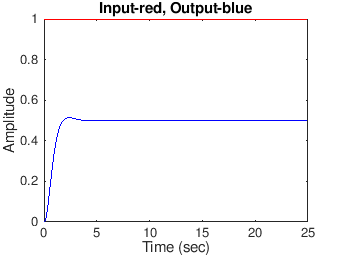
\includegraphics [scale=0.6]{fig1}
\caption{Respuesta con K = 1. Se aprecia error de estado estacionario igual a 0.5}
\end{figure}
\end{block}
\end{frame}


\begin{frame}{Pregunta 34}{Respuesta en el tiempo}
\begin{block}{Código de MATLAB}
\begin{figure}[h!]
\centering
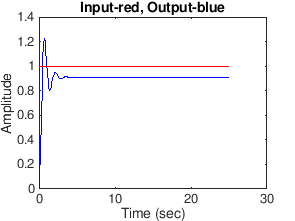
\includegraphics [scale=0.6]{fig2}
\caption{Respuesta con K = 10. Se aprecia error de estado estacionario de 0.1 aproximadamente}
\end{figure}
\end{block}
\end{frame}

\begin{frame}{Pregunta 34}{Respuesta en el tiempo}
\begin{block}{Código de MATLAB}
\begin{figure}[h!]
\centering
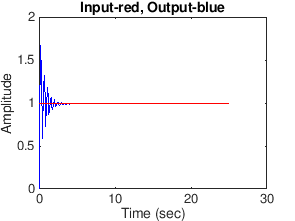
\includegraphics [scale=0.6]{fig3}
\caption{Respuesta con K = 100. Se aprecia error de estado estacionario pequeño.}
\end{figure}
\end{block}
\end{frame}

\begin{frame}{Pregunta 34}{Respuesta en el tiempo}
\begin{block}{Código de MATLAB}
\begin{figure}[h!]
\centering
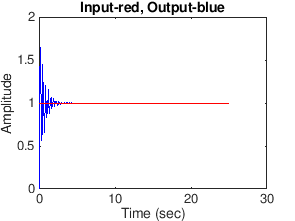
\includegraphics [scale=0.6]{fig4}
\caption{Respuesta con K = 1000. Se aprecia error de estado estacionario muy pequeño.}
\end{figure}
\end{block}
\end{frame}

%%%%%%%%%%%%%%%%%%%%%%%%%%%%5
\section{Información de contacto}
% contact information
\begin{frame}{Feedback}{Información de contacto}
En caso de comentarios, sugerencias o dudas, no dudes en contactarme.
  \begin{center}
    \insertauthor\\
    \chref{https://mixlaab.github.io}{https://mixlaab.github.io}\\
    WA: 8119022700\\
    %9220 Aalborg Ø
  \end{center}
\end{frame}
%%%%%%%%%%%%%%%%

{\aauwavesbg%
\begin{frame}[plain,noframenumbering]%
  \finalpage{Fin}
\end{frame}}
%%%%%%%%%%%%%%%%

\end{document}
